
\section{Olá Mundo}

Tudo pronto para criar seu primeiro programa em SuperCollider? Assumindo que você tem o SC aberto e funcionando à sua frente, abra um novo documento (menu File$\rightarrow$New ("Arquivo$\rightarrow$Novo") ou o atalho [ctrl+N]) e digite a seguinte linha:

 
\begin{lstlisting}[style=SuperCollider-IDE, basicstyle=\scttfamily\footnotesize ]
"Olá Mundo".postln;
\end{lstlisting}
 
Posicione o cursor em qualquer lugar desta linha (não importa se início, meio ou fim). Pressione [ctrl+Enter] para executar o código. "Olá Mundo" aparece no seu Post window ("Janela de postagem"). Parabéns! Este foi seu primeiro programa em SuperCollider.

 
\bigskip
\todo[inline, color=green!40]{ DICA: Em todo este livro, ctrl (control) indica a tecla modificadora para atalhos de teclado que é usada nas plataformas Linux e Windows. No Mac OSX, use a tecla command (cmd). }
\bigskip
 

A figura \ref{fig:scidegui} mostra uma foto de tela do IDE (Integrated Development Environment ou "Ambiente de desenvolvimento integrado") do SuperCollider no momento em que é aberto. Vamos agora nos familiarizar com essa interface.

\begin{figure}[t]
\centerline{\framebox{
	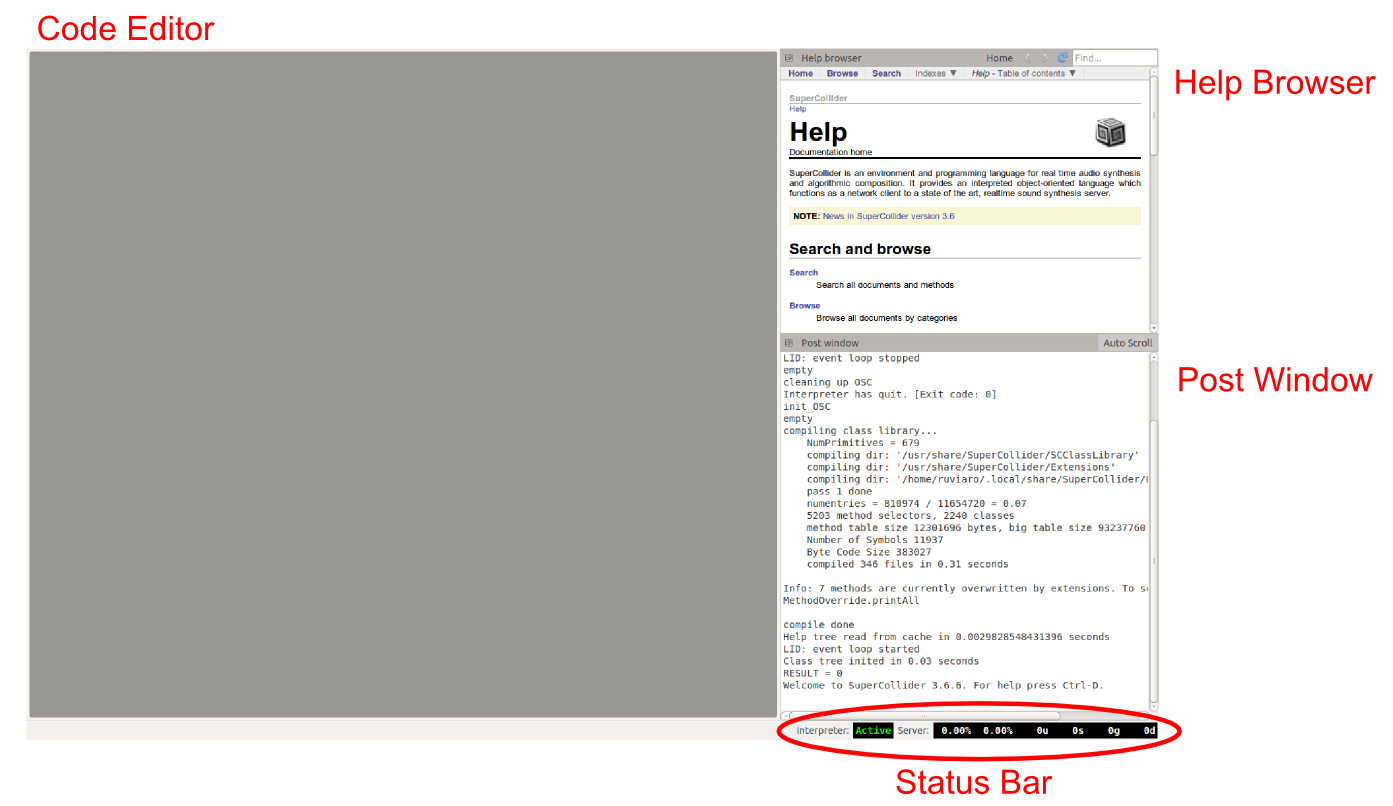
\includegraphics[width=0.7\columnwidth]{fig-supercollider-ide-2.png}}}
\caption{A interface IDE do SuperCollider.}
\label{fig:scidegui}
\end{figure}

O que é o IDE do SuperCollider? É um "ambiente de programação multiplataforma desenvolvido especificamente para o SuperCollider (\dots), 
fácil de começar a usar, prático de lidar e dotado de recursos poderosos para programadores experientes. Ele também é bastante personalizável. Roda igualmente bem e tem quase a mesma aparência no 
Mac OSX, Linux e Windows."\footnote{Citado da documentação do SuperCollider: \url{http://doc.sccode.org/Guides/SCIde.html}. Visite esta página para aprender mais sobre a interface do IDE.}

As principais partes que você vê são o Editor de Código, o Navegador de Ajuda ("Help browser") e a Janela de Postagem ("Post window"). Se você não estiver vendo qualquer uma dessas quando abrir o Super Collider, simplesmente vá para o menu View$\rightarrow$Docklets (é onde você pode exibir ou esconder cada uma delas). Há também a Barra de Status, sempre localizada no canto inferior direito da janela.

Sempre mantenha a Post window visível, mesmo se você ainda não entender todas as coisas que são mostradas ali. A Post window mostra as reações do programa aos seus comandos: resultados da execução de códigos, notificações diversas, avisos, erros, etc.

\bigskip
\todo[inline, color=green!40]{ 
DICA: Você pode aumentar ou reduzir temporariamente o tamanho da fonte do editor com os atalhos [Ctrl++] e [Ctrl+-] (ou seja, a tecla control junto com as teclas de mais ou menos, respectivamente). Se você está em um laptop que não tem uma tecla + de verdade, use [Ctrl+shift+=].}
\bigskip


